\begin{frame}[t] \frametitle{Tool calling}
\framesubtitle{Descrizione}
{\footnotesize
\onslide<1->
    \begin{minipage}[t]{\textwidth}
        \begin{itemize}[leftmargin=10pt,align=right]
            \item[\alert{\faArrowCircleRight}] Tecnica di mitigazione della \textit{knowledge cut-off}\ldots
            \item[\alert{\faArrowCircleRight}] \ldots ma non solo
            \onslide<2->\begin{itemize}[leftmargin=10pt,align=right]
                \item[\alert{\faArrowCircleRight}] Ricerca di informazioni non presenti nella sua base di conoscenza (es. ``Che tempo fa a Venezia?'')
                \onslide<3->\item[\alert{\faExclamationTriangle}] Quindi, differenza con RAG \textit{web search}...?! 
                \onslide<4->\item[\alert{\faArrowCircleRight}] Messa in atto di ciò che comprende
                \begin{itemize}[leftmargin=10pt,align=right]
                    \item[\alert{\faArrowCircleRight}] ``Prenota un biglietto''
                    \item[\alert{\faArrowCircleRight}] ``Invia un'email''
                    \item[\alert{\faArrowCircleRight}] ``Crea un nuovo \textit{ticket} di segnalazione guasto''
                \end{itemize}    
                \onslide<5->\item[\alert{\faArrowCircleRight}] Primo passaggio nella transizione da LLM a \alert{ALM} (Action Language Model)
            \end{itemize}
        \end{itemize}
    \end{minipage}
}
\end{frame}
%
\begin{frame}[t] \frametitle{Tool calling}
\framesubtitle{Differenze con RAG}
{\small
\onslide<1->
    \begin{minipage}[t]{\textwidth}
        {\footnotesize
            \begin{table}
                \renewcommand{\arraystretch}{1.3}
                \centering
                \begin{tabularx}{\textwidth}{Xp{5.5cm}}
                    \toprule
                    \textbf{Tool Calling} & \textbf{RAG}\\
                    \midrule
                    Chiamare un idraulico per riparare una perdita & Leggere un manuale fai-da-te per risolverla da solo\\
                    \midrule
                    ``In base a quello che mi hai chiesto, ecco come far agire il sistema con i mezzi a disposizione'' & ``In base a quello che mi hai chiesto e avendo letto alcuni documenti, ti spiego''\\
                    \midrule
                    Esegue azioni dal vivo o recupera dati dal vivo & Si concentra sulla generazione delle risposte utilizzando contenuti recuperati\\
                    \midrule                    
                    Richiede all'\textit{app client} di eseguire il \textit{tool} & Recupera solo documenti e continua a generare la risposta\\
                    \bottomrule
                \end{tabularx}
            \end{table}
        }
    \end{minipage}
}
\end{frame}
%
\begin{frame}[fragile,t] \frametitle{Tool calling}
\framesubtitle{Componenti chiave in Spring AI}
{\scriptsize
    \vspace*{-.7cm}
    \begin{minipage}[t]{\textwidth}
        \begin{block}{Classe di definizione dei \textit{tool}}
		    {\tiny\inputminted{java}{code/TimeTools.java}}
        \end{block}
        \only<2-4|handout:1>{
        \vspace*{.3cm}
        \begin{itemize}[leftmargin=10pt,align=right]
            \onslide<2->\item[\alert{\faArrowCircleRight}] Solitamente istanziati come \alert{\texttt{@Component}}
            \onslide<3->\item[\alert{\faArrowCircleRight}] Ogni metodo a disposizione del LLM come \textit{tool} deve essere annotato come \alert{\texttt{@Tool}}
            \onslide<4->\begin{itemize}[leftmargin=10pt,align=right]
                \item[\alert{\faArrowCircleRight}] se \texttt{name} non specificato, Spring AI popola il parametro con il nome del metodo
                \item[\alert{\faExclamationTriangle}] \texttt{name} come \alert{identificativo univoco} per Spring AI!
                \item[\alert{\faArrowCircleRight}] \texttt{description} fornisce il \alert{contesto} al LLM per determinare se utilizzare il \textit{tool} in base alla richiesta utente!
                \item[\alert{\faArrowCircleRight}] \alert{\texttt{@ToolParam}} fornisce ulteriore contesto al LLM per iniettare parametri al metodo
            \end{itemize}
        \end{itemize}
        }
        \hspace*{2cm}
        \only<5|handout:2>{
        \begin{minipage}[t]{.8\textwidth}
			\renewcommand{\epigraphsize}{\scriptsize}
			\setlength{\afterepigraphskip}{5pt}
			\setlength{\beforeepigraphskip}{0pt}
			\setlength{\epigraphwidth}{\textwidth}
			\epigraph{\textit{\alert{\faUser} ``D: Che ore sono a New York?''\\
			\alert{\faTerminal\ (thinking)} --- Scansiono i tool a disposizione\ldots ---\\
            \alert{\faTerminal\ (thinking)} --- Vedo che ho dei tool che gestiscono il recupero dell'ora\ldots ---\\
            \alert{\faTerminal\ (thinking)} --- Il primo tool è relativo alla posizione dell'utente\ldots ---\\
            \alert{\faTerminal\ (thinking)} --- Il secondo tool è più astratto e determina la posizione attraverso parametrizzazione del fuso orario\ldots ---\\
            \alert{\faTerminal\ (thinking)} --- \ldots Il fuso orario di New York è America/New York\ldots ---\\
			\alert{\faTerminal} ``R: Utilizza il tool \texttt{getCurrentTime('America/New York')}.''}}{\textbf{Processo di \textit{method as tool}}}
        \end{minipage}
        }
    \end{minipage}
}
\end{frame}
%
\begin{frame}[fragile,t] \frametitle{Tool calling}
\framesubtitle{Componenti chiave in Spring AI}
{\footnotesize
    \vspace*{-.7cm}
    \begin{minipage}[t]{\textwidth}
        \begin{block}{\texttt{ChatClient} potenziato con \textit{tool}}
		    {\tiny\inputminted{java}{code/ToolConfig.java}}
        \end{block}
        \vspace*{.3cm}
        \begin{itemize}[leftmargin=10pt,align=right]
            \onslide<1->\item[\alert{\faArrowCircleRight}] Disponibilità dei \textit{tool} al \texttt{ChatClient} attraverso \textit{injection}
        \end{itemize}
    \end{minipage}
}
\end{frame}
%
\begin{frame}[fragile,t] \frametitle{Tool calling}
\framesubtitle{Workflow}
\vspace*{-.7cm}
{\footnotesize
    \begin{itemize}
        \only<1|handout:1>{\item[\alertedcircled{1}] L'utente invia la richiesta al LLM attraverso \texttt{ChatClient}/\texttt{ChatModel} riferendo al LLM i \textit{tool} a sua disposizione}
        \only<2|handout:2>{\item[\alertedcircled{2}] Se il LLM decide di chiamare un \textit{tool}, invia una \textit{response} con nome del \textit{tool} e parametri istanziati, seguendo la schema definito da \texttt{@Tool} e \texttt{@ToolParam}}
        \only<3|handout:3>{\item[\alertedcircled{3}] L'applicativo interroga il \texttt{@Bean} corrispondente alla classe che contiene il metodo con i parametri istanziati suggeriti dal LLM}
        \only<4|handout:4>{\item[\alertedcircled{4}] Il \texttt{@Bean} invoca il metodo con i parametri restituiti dal LLM e restituisce il risultato al \textit{container} Spring}
        \only<5|handout:5>{\item[\alertedcircled{5}] Il sistema invoca nuovamente il LLM con la richiesta utente precedente ma ulteriormente contestualizzata dall'\textit{output} del \textit{tool}}
        \only<6|handout:6>{\item[\alertedcircled{6}] Il LLM restituisce la risposta finale al \texttt{ChatClient}/\texttt{ChatModel} sfruttando generazione di testo e contesto}
    \end{itemize}
    }
\vfill
\begin{figure}[ht]
    \centering
    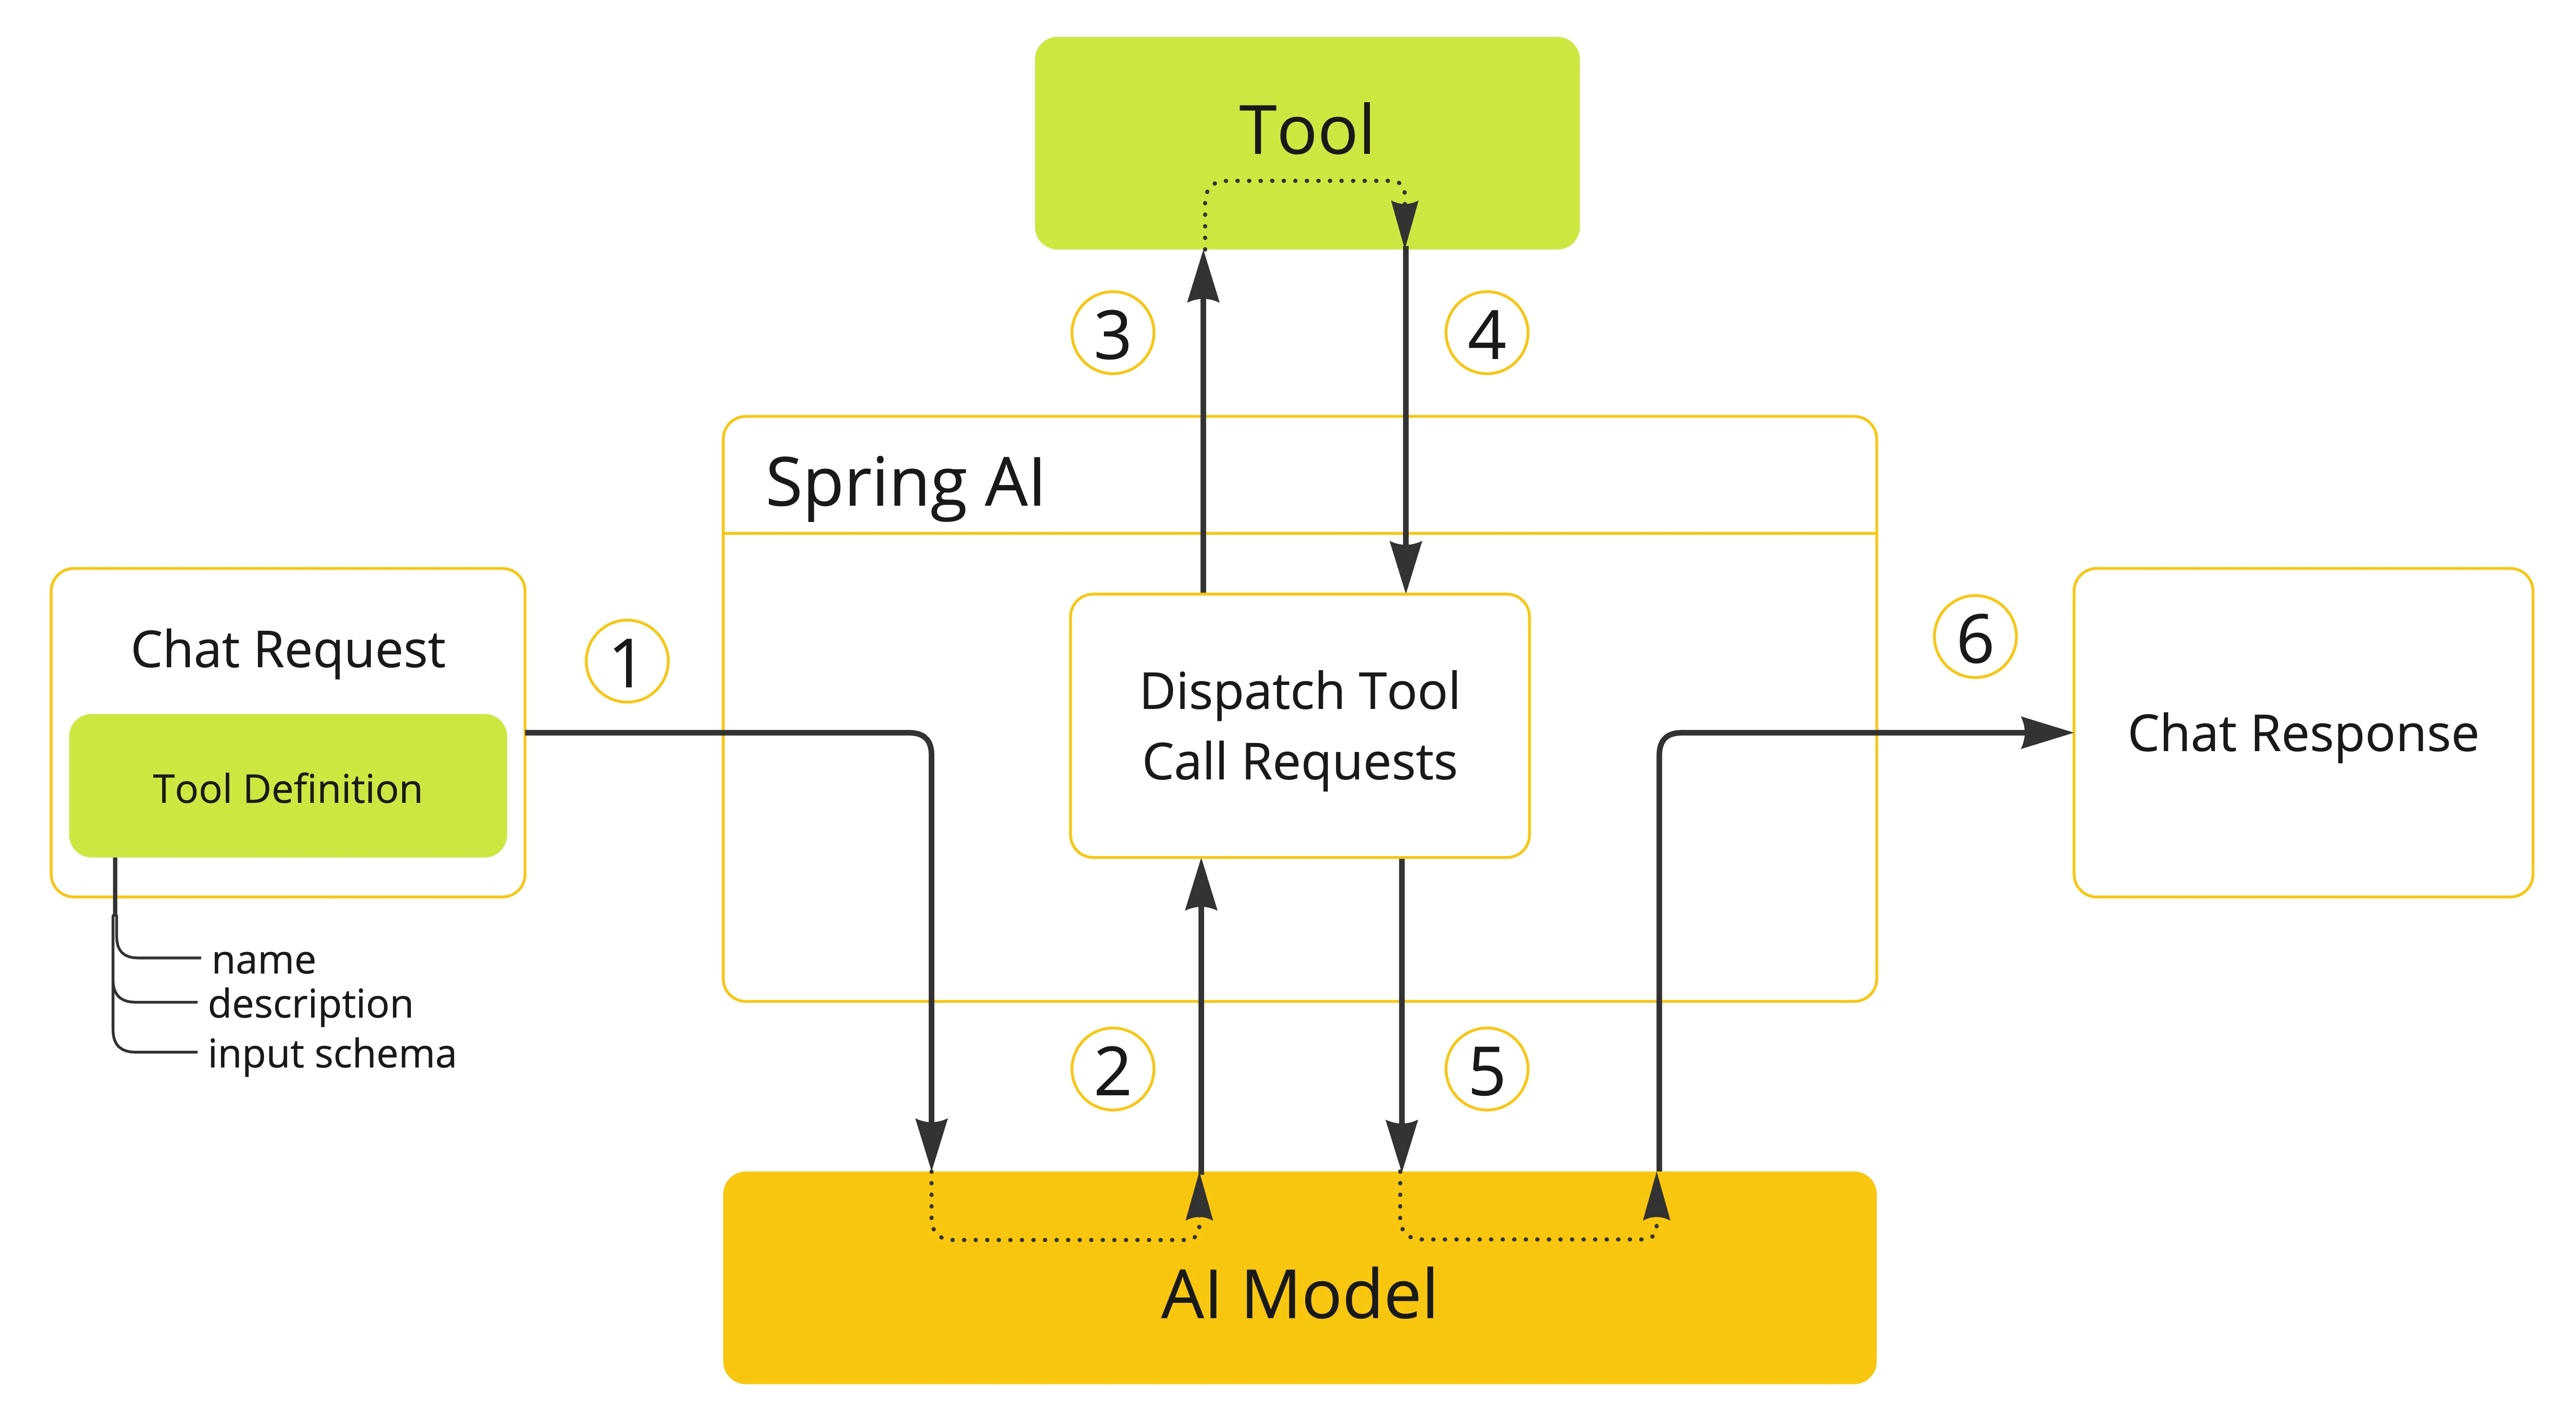
\includegraphics[width=\textwidth]{img/tool-calling.png}
    {\tiny\\\textit{\textcopyright Spring AI}}
\end{figure}

\end{frame}
%